\documentclass[]{article}
\usepackage{lmodern}
\usepackage{amssymb,amsmath}
\usepackage{ifxetex,ifluatex}
\usepackage{fixltx2e} % provides \textsubscript
\ifnum 0\ifxetex 1\fi\ifluatex 1\fi=0 % if pdftex
  \usepackage[T1]{fontenc}
  \usepackage[utf8]{inputenc}
\else % if luatex or xelatex
  \ifxetex
    \usepackage{mathspec}
  \else
    \usepackage{fontspec}
  \fi
  \defaultfontfeatures{Ligatures=TeX,Scale=MatchLowercase}
\fi
% use upquote if available, for straight quotes in verbatim environments
\IfFileExists{upquote.sty}{\usepackage{upquote}}{}
% use microtype if available
\IfFileExists{microtype.sty}{%
\usepackage{microtype}
\UseMicrotypeSet[protrusion]{basicmath} % disable protrusion for tt fonts
}{}
\usepackage[margin=1in]{geometry}
\usepackage{hyperref}
\hypersetup{unicode=true,
            pdftitle={Homework 3},
            pdfauthor={Nick Bruns, Zeyi Han, Shubhi Sharma, Maggie Swift},
            pdfborder={0 0 0},
            breaklinks=true}
\urlstyle{same}  % don't use monospace font for urls
\usepackage{color}
\usepackage{fancyvrb}
\newcommand{\VerbBar}{|}
\newcommand{\VERB}{\Verb[commandchars=\\\{\}]}
\DefineVerbatimEnvironment{Highlighting}{Verbatim}{commandchars=\\\{\}}
% Add ',fontsize=\small' for more characters per line
\usepackage{framed}
\definecolor{shadecolor}{RGB}{248,248,248}
\newenvironment{Shaded}{\begin{snugshade}}{\end{snugshade}}
\newcommand{\AlertTok}[1]{\textcolor[rgb]{0.94,0.16,0.16}{#1}}
\newcommand{\AnnotationTok}[1]{\textcolor[rgb]{0.56,0.35,0.01}{\textbf{\textit{#1}}}}
\newcommand{\AttributeTok}[1]{\textcolor[rgb]{0.77,0.63,0.00}{#1}}
\newcommand{\BaseNTok}[1]{\textcolor[rgb]{0.00,0.00,0.81}{#1}}
\newcommand{\BuiltInTok}[1]{#1}
\newcommand{\CharTok}[1]{\textcolor[rgb]{0.31,0.60,0.02}{#1}}
\newcommand{\CommentTok}[1]{\textcolor[rgb]{0.56,0.35,0.01}{\textit{#1}}}
\newcommand{\CommentVarTok}[1]{\textcolor[rgb]{0.56,0.35,0.01}{\textbf{\textit{#1}}}}
\newcommand{\ConstantTok}[1]{\textcolor[rgb]{0.00,0.00,0.00}{#1}}
\newcommand{\ControlFlowTok}[1]{\textcolor[rgb]{0.13,0.29,0.53}{\textbf{#1}}}
\newcommand{\DataTypeTok}[1]{\textcolor[rgb]{0.13,0.29,0.53}{#1}}
\newcommand{\DecValTok}[1]{\textcolor[rgb]{0.00,0.00,0.81}{#1}}
\newcommand{\DocumentationTok}[1]{\textcolor[rgb]{0.56,0.35,0.01}{\textbf{\textit{#1}}}}
\newcommand{\ErrorTok}[1]{\textcolor[rgb]{0.64,0.00,0.00}{\textbf{#1}}}
\newcommand{\ExtensionTok}[1]{#1}
\newcommand{\FloatTok}[1]{\textcolor[rgb]{0.00,0.00,0.81}{#1}}
\newcommand{\FunctionTok}[1]{\textcolor[rgb]{0.00,0.00,0.00}{#1}}
\newcommand{\ImportTok}[1]{#1}
\newcommand{\InformationTok}[1]{\textcolor[rgb]{0.56,0.35,0.01}{\textbf{\textit{#1}}}}
\newcommand{\KeywordTok}[1]{\textcolor[rgb]{0.13,0.29,0.53}{\textbf{#1}}}
\newcommand{\NormalTok}[1]{#1}
\newcommand{\OperatorTok}[1]{\textcolor[rgb]{0.81,0.36,0.00}{\textbf{#1}}}
\newcommand{\OtherTok}[1]{\textcolor[rgb]{0.56,0.35,0.01}{#1}}
\newcommand{\PreprocessorTok}[1]{\textcolor[rgb]{0.56,0.35,0.01}{\textit{#1}}}
\newcommand{\RegionMarkerTok}[1]{#1}
\newcommand{\SpecialCharTok}[1]{\textcolor[rgb]{0.00,0.00,0.00}{#1}}
\newcommand{\SpecialStringTok}[1]{\textcolor[rgb]{0.31,0.60,0.02}{#1}}
\newcommand{\StringTok}[1]{\textcolor[rgb]{0.31,0.60,0.02}{#1}}
\newcommand{\VariableTok}[1]{\textcolor[rgb]{0.00,0.00,0.00}{#1}}
\newcommand{\VerbatimStringTok}[1]{\textcolor[rgb]{0.31,0.60,0.02}{#1}}
\newcommand{\WarningTok}[1]{\textcolor[rgb]{0.56,0.35,0.01}{\textbf{\textit{#1}}}}
\usepackage{graphicx,grffile}
\makeatletter
\def\maxwidth{\ifdim\Gin@nat@width>\linewidth\linewidth\else\Gin@nat@width\fi}
\def\maxheight{\ifdim\Gin@nat@height>\textheight\textheight\else\Gin@nat@height\fi}
\makeatother
% Scale images if necessary, so that they will not overflow the page
% margins by default, and it is still possible to overwrite the defaults
% using explicit options in \includegraphics[width, height, ...]{}
\setkeys{Gin}{width=\maxwidth,height=\maxheight,keepaspectratio}
\IfFileExists{parskip.sty}{%
\usepackage{parskip}
}{% else
\setlength{\parindent}{0pt}
\setlength{\parskip}{6pt plus 2pt minus 1pt}
}
\setlength{\emergencystretch}{3em}  % prevent overfull lines
\providecommand{\tightlist}{%
  \setlength{\itemsep}{0pt}\setlength{\parskip}{0pt}}
\setcounter{secnumdepth}{0}
% Redefines (sub)paragraphs to behave more like sections
\ifx\paragraph\undefined\else
\let\oldparagraph\paragraph
\renewcommand{\paragraph}[1]{\oldparagraph{#1}\mbox{}}
\fi
\ifx\subparagraph\undefined\else
\let\oldsubparagraph\subparagraph
\renewcommand{\subparagraph}[1]{\oldsubparagraph{#1}\mbox{}}
\fi

%%% Use protect on footnotes to avoid problems with footnotes in titles
\let\rmarkdownfootnote\footnote%
\def\footnote{\protect\rmarkdownfootnote}

%%% Change title format to be more compact
\usepackage{titling}

% Create subtitle command for use in maketitle
\providecommand{\subtitle}[1]{
  \posttitle{
    \begin{center}\large#1\end{center}
    }
}

\setlength{\droptitle}{-2em}

  \title{Homework 3}
    \pretitle{\vspace{\droptitle}\centering\huge}
  \posttitle{\par}
    \author{Nick Bruns, Zeyi Han, Shubhi Sharma, Maggie Swift}
    \preauthor{\centering\large\emph}
  \postauthor{\par}
      \predate{\centering\large\emph}
  \postdate{\par}
    \date{2/10/2020}


\begin{document}
\maketitle

\emph{Exercise 1.} Is the infection rate estimated to be higher for
survivors or for those that die? How are these two distributions
affected by the underlying prevalence of infection, θ?

Yes. An increase in theta leads to more death (maximum value for the
distribution shift right). Increasing theta also leads to decreased
survival (maximum shift left, and with decreasing probability)

\begin{Shaded}
\begin{Highlighting}[]
\NormalTok{n <-}\StringTok{ }\DecValTok{100}
\NormalTok{pi0 <-}\StringTok{ }\FloatTok{0.8}  \CommentTok{#[S|I=1]}
\NormalTok{pi1 <-}\StringTok{ }\FloatTok{0.2}   \CommentTok{#[S|I=0]}
\NormalTok{theta <-}\StringTok{ }\FloatTok{0.03}   \CommentTok{# new infected}
 
\KeywordTok{par}\NormalTok{(}\DataTypeTok{mfrow =} \KeywordTok{c}\NormalTok{(}\DecValTok{2}\NormalTok{,}\DecValTok{2}\NormalTok{))}
\NormalTok{IS0 <-}\StringTok{ }\KeywordTok{dbinom}\NormalTok{(}\DecValTok{1}\OperatorTok{:}\NormalTok{n, }\DecValTok{100}\NormalTok{, (}\DecValTok{1}\OperatorTok{-}\NormalTok{pi0)}\OperatorTok{*}\NormalTok{theta}\OperatorTok{/}\NormalTok{((}\DecValTok{1}\OperatorTok{-}\NormalTok{pi0)}\OperatorTok{*}\NormalTok{(}\DecValTok{1}\OperatorTok{-}\NormalTok{theta)}\OperatorTok{+}\StringTok{ }\NormalTok{(}\DecValTok{1}\OperatorTok{-}\NormalTok{pi1)}\OperatorTok{*}\NormalTok{theta))}
\KeywordTok{plot}\NormalTok{(}\DecValTok{1}\OperatorTok{:}\DecValTok{100}\NormalTok{, IS0)}
 
\NormalTok{IS1 <-}\StringTok{ }\KeywordTok{dbinom}\NormalTok{(}\DecValTok{1}\OperatorTok{:}\NormalTok{n, }\DecValTok{100}\NormalTok{, pi1}\OperatorTok{*}\NormalTok{theta}\OperatorTok{/}\NormalTok{(pi0}\OperatorTok{*}\NormalTok{(}\DecValTok{1}\OperatorTok{-}\NormalTok{theta)}\OperatorTok{+}\StringTok{ }\NormalTok{pi}\OperatorTok{*}\NormalTok{theta))}
\KeywordTok{plot}\NormalTok{(}\DecValTok{1}\OperatorTok{:}\DecValTok{100}\NormalTok{, IS1)}

\NormalTok{theta <-}\StringTok{ }\FloatTok{0.8}
\NormalTok{IS0_}\DecValTok{2}\NormalTok{ <-}\StringTok{ }\KeywordTok{dbinom}\NormalTok{(}\DecValTok{1}\OperatorTok{:}\NormalTok{n, }\DecValTok{100}\NormalTok{, (}\DecValTok{1}\OperatorTok{-}\NormalTok{pi0)}\OperatorTok{*}\NormalTok{theta}\OperatorTok{/}\NormalTok{((}\DecValTok{1}\OperatorTok{-}\NormalTok{pi0)}\OperatorTok{*}\NormalTok{(}\DecValTok{1}\OperatorTok{-}\NormalTok{theta)}\OperatorTok{+}\StringTok{ }\NormalTok{(}\DecValTok{1}\OperatorTok{-}\NormalTok{pi1)}\OperatorTok{*}\NormalTok{theta))}
\KeywordTok{plot}\NormalTok{(}\DecValTok{1}\OperatorTok{:}\DecValTok{100}\NormalTok{, IS0_}\DecValTok{2}\NormalTok{)}
 
\NormalTok{IS1_}\DecValTok{2}\NormalTok{ <-}\StringTok{ }\KeywordTok{dbinom}\NormalTok{(}\DecValTok{1}\OperatorTok{:}\NormalTok{n, }\DecValTok{100}\NormalTok{, pi1}\OperatorTok{*}\NormalTok{theta}\OperatorTok{/}\NormalTok{(pi0}\OperatorTok{*}\NormalTok{(}\DecValTok{1}\OperatorTok{-}\NormalTok{theta)}\OperatorTok{+}\StringTok{ }\NormalTok{pi}\OperatorTok{*}\NormalTok{theta))}
\KeywordTok{plot}\NormalTok{(}\DecValTok{1}\OperatorTok{:}\DecValTok{100}\NormalTok{, IS1_}\DecValTok{2}\NormalTok{)}
\end{Highlighting}
\end{Shaded}

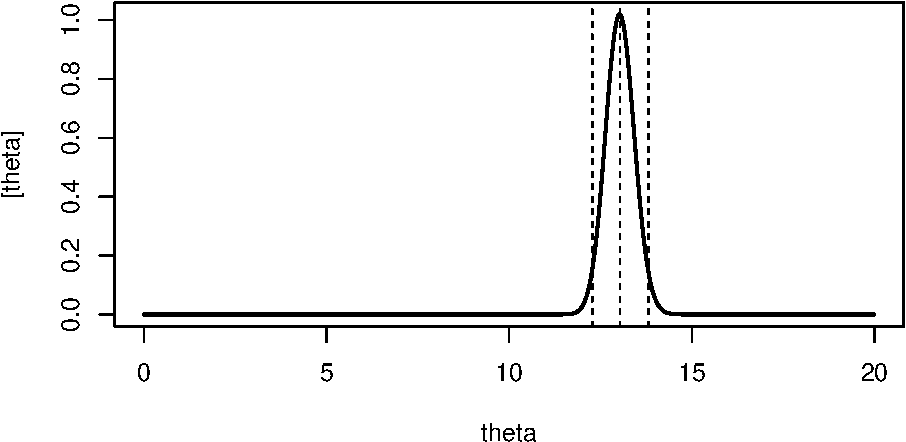
\includegraphics{HW3_files/figure-latex/unnamed-chunk-1-1.pdf}

\emph{Exercise 2.} The variance in beta distribution decreases as the
value of parameter b increases. Change parameter values to demonstrate
this with a plot. Then compare the mean and variance (see Appendix) from
the moments for the binomial and beta-binomial.

Variance decreases with increasing beta.

\emph{Exercise 3.} I observe \(D\) and \(S\), and I know \(\phi\) from
previous studies. What is the probability of an observation
\([D=1,S=1]\). (Hint: use total probability on \([D,I,S]\). Now write
down the posterior distribution for a parameter that represents the
product of infection and survival \(\rho=\theta\pi_1\) given
observations and known detection probability, i.e.,
\([\rho|D=1,S=1,\phi]\).

\emph{Exercise 4.} Write a function to determine the posterior estimate
of the mean for a normal likelihood, normal prior distribution, and
known variance \(\sigma^2\). You will need to generate a sample, supply
a prior mean and variance, determine the posterior mean and variance,
and plot.

\begin{Shaded}
\begin{Highlighting}[]
\NormalTok{posteriorSample <-}\StringTok{ }\ControlFlowTok{function}\NormalTok{(samples, llMean, priorMean, llVar, priorVar)\{}

\CommentTok{#data  }
\NormalTok{n =}\StringTok{ }\NormalTok{samples}
\NormalTok{mu =}\StringTok{ }\NormalTok{llMean}
\NormalTok{mu0 =}\StringTok{ }\NormalTok{priorMean}
\NormalTok{sigma =}\StringTok{ }\NormalTok{llVar}
\NormalTok{tau =}\StringTok{ }\NormalTok{priorVar }

\KeywordTok{set.seed}\NormalTok{(}\DecValTok{101}\NormalTok{)}

\CommentTok{#sampling}
\NormalTok{y <-}\StringTok{ }\KeywordTok{rnorm}\NormalTok{(n, mu, sigma)}
\NormalTok{ybar <-}\StringTok{ }\KeywordTok{mean}\NormalTok{(y)}

\NormalTok{prior <-}\StringTok{ }\KeywordTok{rnorm}\NormalTok{(n, mu0, tau)}

\NormalTok{sigmaN <-}\StringTok{ }\NormalTok{n}\OperatorTok{/}\NormalTok{sigma}\OperatorTok{^}\DecValTok{2} \OperatorTok{+}\StringTok{ }\DecValTok{1}\OperatorTok{/}\NormalTok{tau}\OperatorTok{^}\DecValTok{2}
\NormalTok{muN <-}\StringTok{ }\NormalTok{((n}\OperatorTok{*}\NormalTok{ybar)}\OperatorTok{/}\NormalTok{sigma}\OperatorTok{^}\DecValTok{2} \OperatorTok{+}\StringTok{ }\NormalTok{mu0}\OperatorTok{/}\NormalTok{tau}\OperatorTok{^}\DecValTok{2}\NormalTok{)}\OperatorTok{/}\NormalTok{sigmaN}

\NormalTok{posterior <-}\StringTok{ }\KeywordTok{rnorm}\NormalTok{(n, muN, sigmaN)}

\KeywordTok{return}\NormalTok{(posterior)}
\NormalTok{\}}
\end{Highlighting}
\end{Shaded}

\emph{Exercise 5.} Obtain the posterior mean and variance for regression
parameters for a simulated data set.

For 1000 samples, \(Y|\mu \sim N(\mu, \sigma^2)\). Setting
\(\mu = 4, \sigma = 10\), \(\mu ~ N(\mu_0, \tau^2)\). Setting
\(mu_0= 4, tau = 20\), we get posterior mean \(= 4.04\) and posterior
variance \(= 100.5\).


\end{document}
